\chapter{Data analysis}
\section{General statistics}
\label{sec:general_statistics}
The data we are working with represents sensor readings over a total of 7 days of airport activity, set in September 2018. \\
The data was filtered beforehand to contain only the measurements that correspond to Bluetooth addresses that are already labelled. These correspond to 7.612.286 readings which we filtered further down to 974.152 measurements, only the ones recorded within the arrival area. Therefore we are left to work with 13.530 unique mobile devices. The labels for those addresses are the following (also seen visualised in \cref{fig:stats_labels}):

\begin{itemize}
	\item 8.045 Staff
	\item 3.574 Manual
	\item 1.633 No-q
	\item 278 Privium
\end{itemize}

\begin{figure}[H]
    \centering
    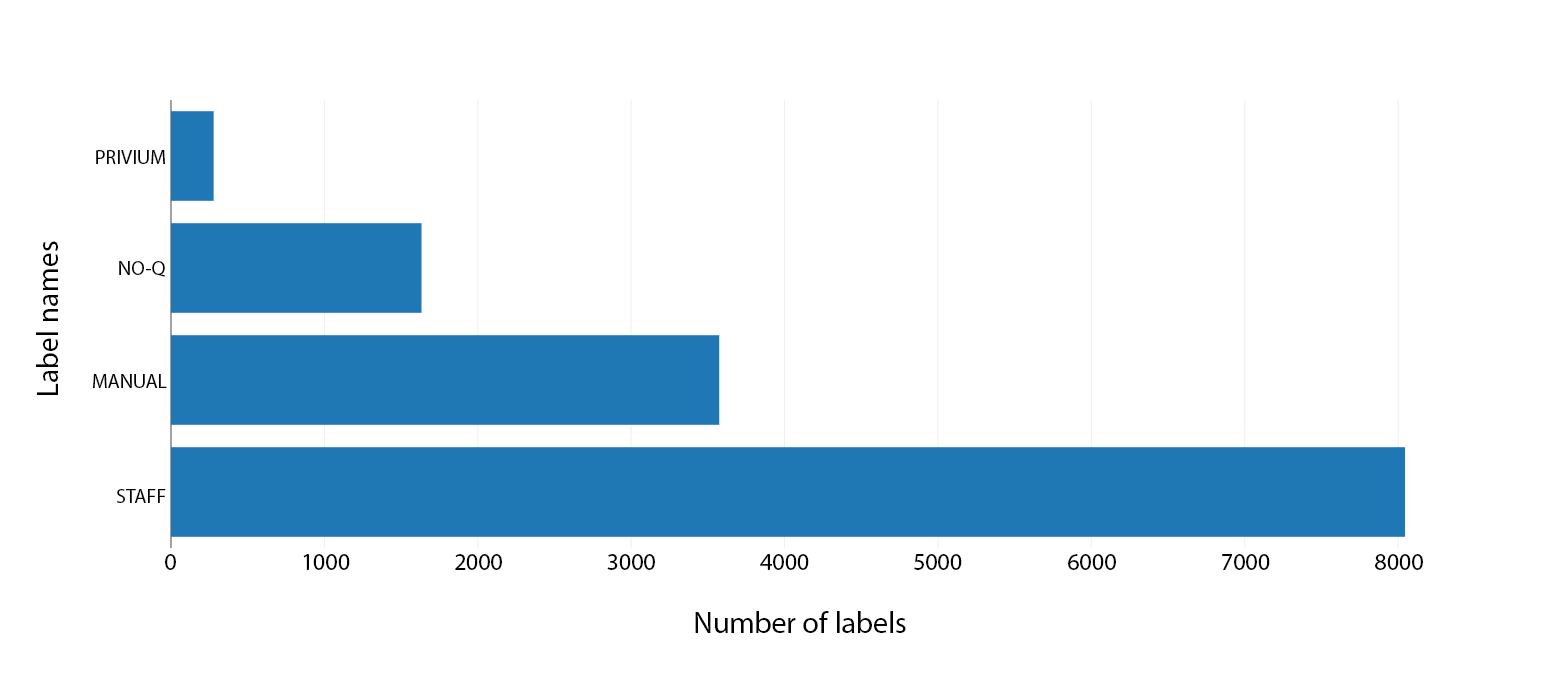
\includegraphics[width=.75\textwidth]{Pictures/Labels.png}
    \caption{Labels}
    \label{fig:stats_labels}
\end{figure}

The value of the signal strength measurements vary between -75 and -3. The value -73 is the most common signal strength, representing 15.34\% of the total measurements. The overall average signal strength is -66.34. This may be seen in \cref{fig:sensor_strength_readings}.\\

\begin{figure}[H]
    \centering
    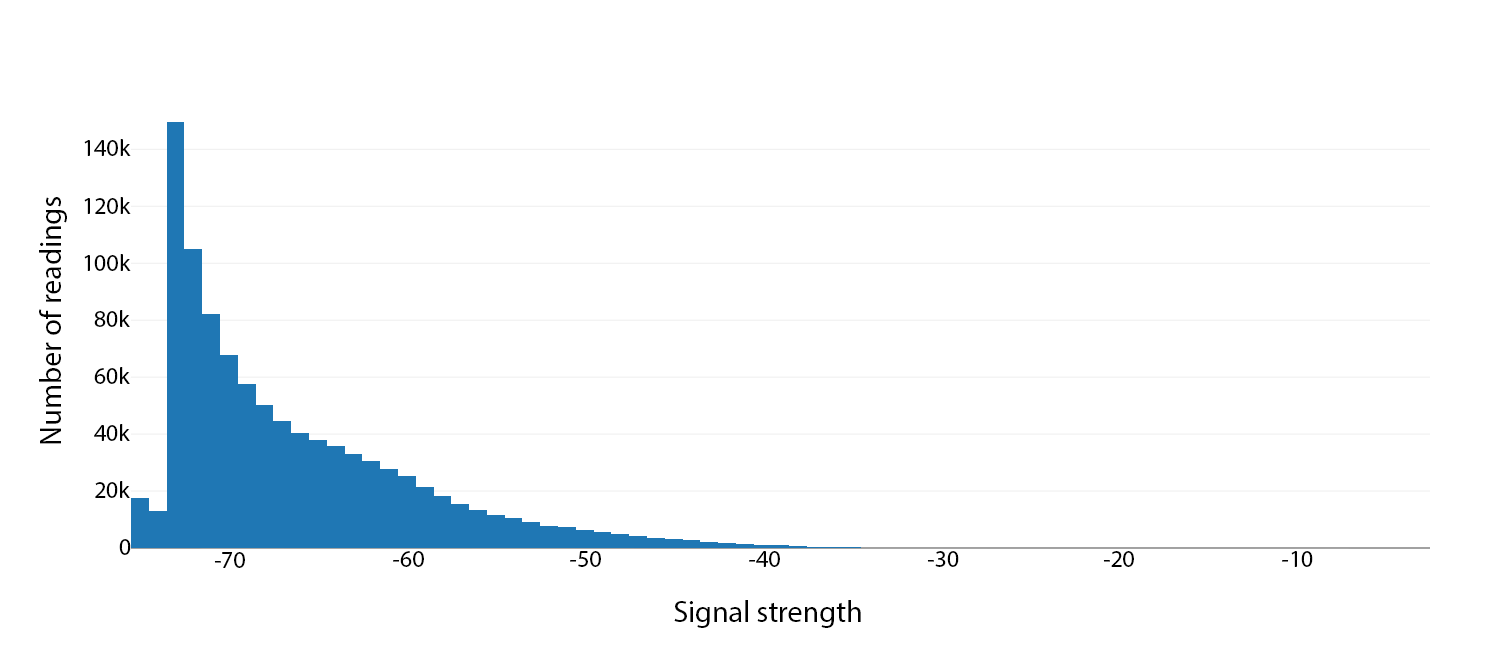
\includegraphics[width=.8\textwidth]{Pictures/Sensor_Strength_Readings.png}
    \caption{Sensor strength readings}
    \label{fig:sensor_strength_readings}
\end{figure}

The chart in \cref{fig:stat:readingspersensor} shows the amount of readings that are taken of members of each class by the different sensors present. The sensor with the most readings is P2 which recorded 88.896 signals. While other nearby sensors have close to that amount of readings, the lowest amount of measurements is from the QE1 sensor that recorded 32.802 signals.\\

\begin{figure}[H]
    \centering
    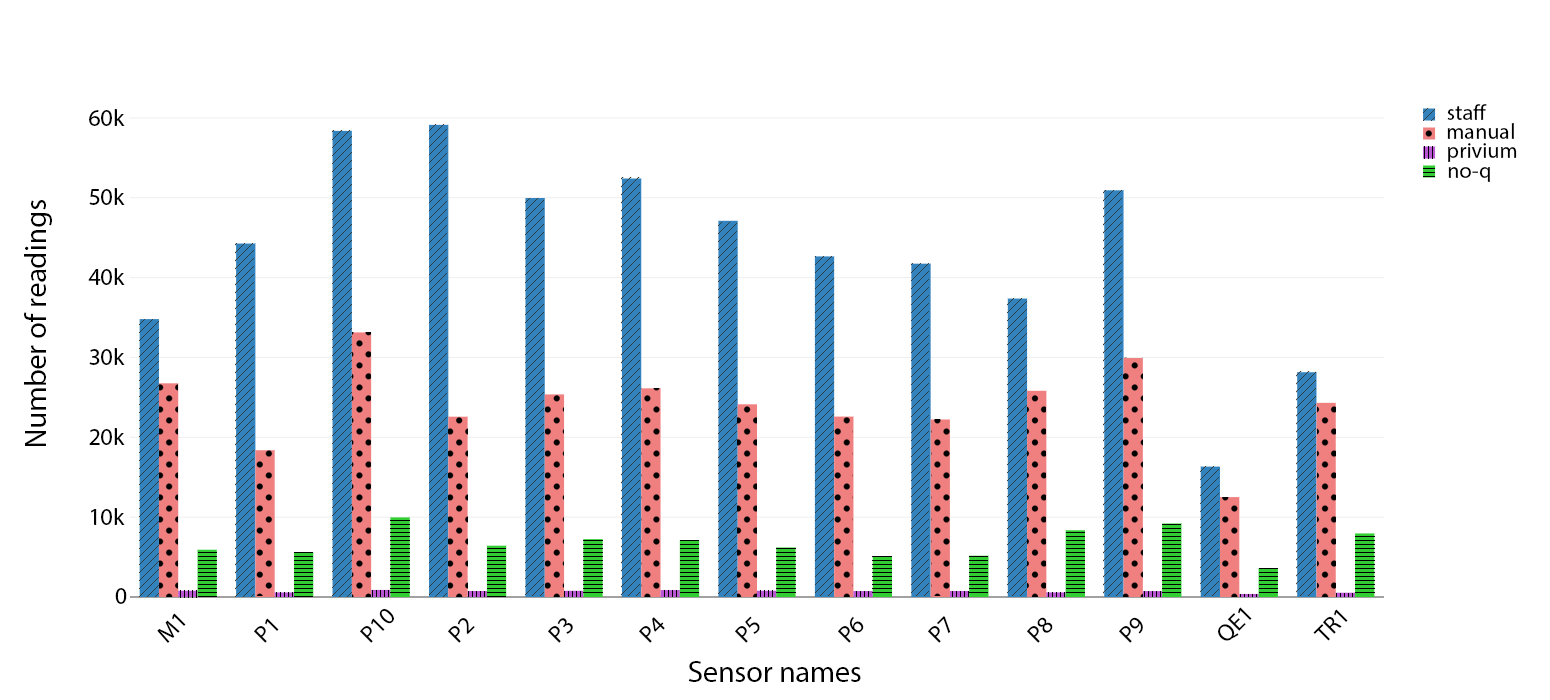
\includegraphics[width=.8\textwidth]{Pictures/Readings_per_sensor.png}
    \caption{Readings per sensor}
    \label{fig:stat:readingspersensor}
\end{figure}

\pagebreak

The distribution in \cref{fig:stat:timespentdistbylabel} displays the amounts of time (in minutes) spent in the area by members of each of the four label groups. We observe that, regardless of label, the majority is in and out in less than 45 minutes.

\begin{figure}[H]
    \centering
    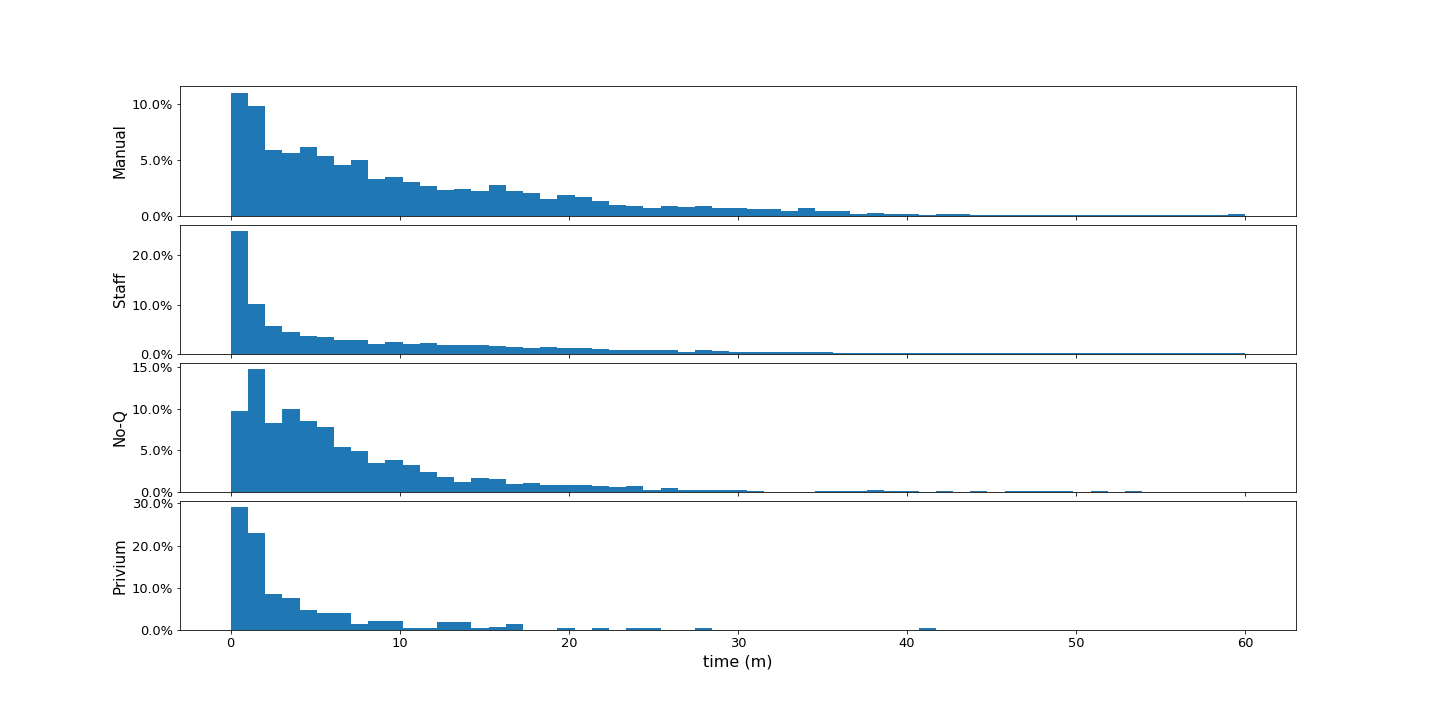
\includegraphics[width=1\textwidth]{Pictures/timespentdistbylabel.png}
    \caption{Distribution of time spent in the area, by label}
    \label{fig:stat:timespentdistbylabel}
\end{figure}

The following percentages represent the ratio of devices in each group that pass through in less than 45 minutes:

\begin{itemize}
	\item Manual:   96.1\%
	\item Staff:    88.9\%
	\item No-Q:     97.6\%
	\item Privium:  95.7\%
\end{itemize}

For example, 96.1\% of addresses labelled as "Manual" take less than 45 minutes to pass.
